



\begin{frame}{\citetitle{MarcoNuno_CongArbEsp_2020_09_01} \footnotemark (1)}
\begin{block}{Detección de conductores autorizados \footnotemark } 
\begin{columns}
\begin{column}{1.0\textwidth}
Se propone un sistema montado en un teléfono inteligente que pueda:
	\begin{itemize}
\item Confirmar de manera continua la identidad de los ocupantes empleando la cámara frontal o posterior
\item Monitorear la ubicación del vehículo mediante el sensor GPS
\item Monitorear cuando el vehículo está en movimiento mediante los acelerómetros
\item Trabajar de manera independiente, conectado continuamente a la corriente y con conexión de datos propia para comunicación externa
	\end{itemize}
\end{column}
\end{columns}
\end{block} 
\footnotetext[1]{\fullcite{MarcoNuno_CongArbEsp_2020_09_01}}
\setcounter{footnote}{0}
\end{frame}


\begin{frame}{\citetitle{MarcoNuno_CongArbEsp_2020_09_01} (2)}
%\begin{block}{Detección de conductores autorizados (2)} 
\begin{columns}
\begin{column}{0.55\textwidth}
Fases de la ejecución:
	\begin{enumerate}
\item Enrolamiento: Los usuarios usan el automovil y sus rostros quedan guardados.
\item Prueba: Se reporta el ingreso de cualquier extraño.
	\end{enumerate}
Limitaciones:
	\begin{itemize}
\item Solo piloto, copiloto y tal vez pasajero viajando en el centro de la parte posterior.
\item Iluminación diurna.
\item Camuflaje en fase temprana.
	\end{itemize}

\end{column}
\begin{column}{0.45\textwidth}
\begin{center}
     %%%%% this is a minipage, so \textwidth is already adjusted to the size of the column
     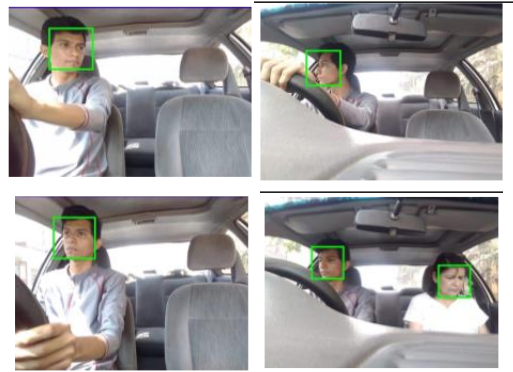
\includegraphics[width=0.99\textwidth]{Figs/ConductorAutorizado1}
     \end{center}
\end{column}

\end{columns}
%\end{block} 
\end{frame}


